\Chapter{Discussion autours des applications cliniques des algorithmes développés}\label{sec:Theme3}

Les deux précédents chapitres ont détaillé les méthodes propres à la généralisation et à l'interprétabilité que nous avons développées.
Dans un cas comme dans l'autre, ce développement est globalement théorique; dans leur structure, application et validation, nos expériences répondent davantage au cahier des charges académique du champs de l'apprentissage machine plutôt qu'aux besoins cliniques. Ce chapitre propose de se détacher de cette logique: il y discute de plusieurs démarches exploratoires que nous avons entreprises pour créer une passerelle entre ces algorithmes et leur utilisation à des fins médicales. Les résultats obtenus étant parfois embryonnaires, cette présentation est avant tout un prétexte à une discussion plus approfondie sur nos travaux. Cela nous ainsi permet d'en illustrer les forces mais aussi les limitations; d'où nous pouvons tirer un certain nombre de recommandations sur les perspectives futures de recherche.
\\
Deux applications seront données en exemple à travers ce chapitre. La première porte sur l'identification du processus de conversion de la Dégénérescence Maculaire Liée à l'Âge (DMLA), du stade non exsudatif vers l'humide. Nos travaux sur la question sont une contribution à une étude menée par l'Hôpital Maisonneuve-Rosemont sur une cohorte de patients recrutée spécifiquement pour cela. \\
La seconde propose un prototype de déploiement d'algorithmes d'assistance au diagnostic à travers une plateforme de visualisation accessible en ligne. Nous y avons déployé nos différents algorithmes et une proposition de mise en forme de ceux-ci. Plus qu'une réelle application, il s'agit d'une démonstration d'un usage possible de ces algorithmes.

\section{Recherche de marqueurs prédictifs de la conversion de la \ac{DMLA}}
 
La DMLA est une maladie largement répandue au sein de la population âgée de 50 ans et plus. Elle survient généralement sous deux formes: le plus fréquente étant la non-exsudative (ou sèche) mais qui peut évoluer sous la forme exsudative (aussi appelée humide ou néovasculaire). La section \ref{sec:DMLADescription} couvre brièvement les principaux marqueurs qui caractérisent un stade ou l'autre de la maladie. Nous renvoyons également vers les travaux de Spaide et al. \cite{spaideConsensusNomenclatureReporting2020}, qui synthétisent la recherche d'un consensus international sur la terminologie derrière la classification de la DMLA et de ses symptômes. L'évolution de la maladie n'est pas symétrique entre les deux yeux; en revanche le patient ayant développé une DMLA exsudative dans un \oeil{} a un risque significativement plus élevé de la développer dans le second \cite{roySecondEyeInvolvement1990, gangnonSeverityAgeRelatedMacular2015}. L'absence de théorie sur le mécanisme de l'évolution de la maladie a motivé plusieurs études sur la question, en particulier sur la prédictibilité algorithmique de la conversion de stade \cite{schmidt-erfurthPredictionIndividualDisease2018, ASCRSPredictionImminent2023, yimPredictingConversionWet2020}. Dans ce contexte là, l'équipe du Docteur Costantino de l'Hôpital Maisonneuve-Rosemont a mis en place un protocole de recrutement et de suivi de patients atteints de DMLA exsudative dans un seul \oeil{} (et donc à risque accru de conversion dans le second). Ces patients sont déjà suivis chaque mois dans le cadre du traitement de l'\oeil{} atteint de DMLA humide (injection intravitréenne d'anti-VEGF), mais dans le cadre de l'étude longitudinale, ils acceptent de se faire imager le second \oeil{}. La spécificité de l'étude repose sur la richesse des acquisitions: au cours de chaque visite, la rétine du patient est visualisée en utilisant:
\begin{itemize}
	\item Une acquisition OCT structurelle prise avec un Spectralis de Heidelberg. Sa résolution est de $96 \times 1024 \times 436$. 
	\item Deux acquisitions OCT structurelles prises avec un Zeiss PLEX, la première couvrant une zone de $3\times 3$mm$^2$ (résolution: $300 \times 300 \times 1536$) et la seconde une zone de $6\times 6$mm$^2$ (résolution: $500 \times 500 \times 1536$)
	\item Originalité de l'étude, le Zeiss PLEX nous fournit également des images OCT angiographiques, de même résolution que celles structurelles. Nous renvoyons à l'annexe \ref{sec:ImagerieRetina}.
\end{itemize}
Chaque acquisition est naturellement centrée sur la macula. Début 2022, la cohorte s'établissait à 118 patients pour un total de 446 visites, soit moins de 4 visites par patients (3.77 en moyenne). Ce chiffre est très faible au regard de la date du début de l'étude (Mars 2019). Il s'explique malheureusement par la pandémie de Covid-19 qui a occasionné une longue interruption dans le suivi de la cohorte.
\\
Sur les 118 patients suivis, 13 ($11\%$) ont développé une DMLA humide dans l'\oeil{} suivi. 
\subsection{Mises en applications des algorithmes et expérimentations}
L'objectif de notre participation à ce projet était de mener une étude préliminaire sur la prédictibilité de la conversion de la DMLA à l'aide des différents algorithmes à notre disposition, notamment ceux développés dans le cadre de cette thèse. Nous souhaitons mentionner ici les expériences conduites à titre d'illustration d'une application réelle mais sans nécessairement rentrer dans le détail de l'implémentation ou des résultats obtenus. Cette précision a son importance car ces travaux sont pour la plupart inachevés ou n'ont pas abouti à des résultats concluants. Cependant, même si les détails ne sont pas donnés ici par concision, l'essentiel des résultats et expérimentations sont consultables sur le billet du blog conçu pour le suivi de ce projet: \url{https://liv4d.github.io/Team_LIV4D.github.io/ophthalmology/oct/amd_progression_prediction/} ou en suivant le QR-code de la figure \ref{fig:blogpost_QRcode}.
\begin{figure}[H]
	\centering
	
\includegraphics[width=0.25\textwidth]{applications/DMLA/DMLA_blog_url}
	\caption{Lien vers le post de blog détaillant les résultats des expériences liées à la DMLA.}
	\label{fig:blogpost_QRcode}
	
\end{figure}

\subsubsection{Classification des B-Scans}
Dans le chapitre \ref{sec:Theme2}, nous avons entraîné différents modèles à détecter différentes pathologies sur des B-scans d'une base de données publiques (correspondant à des OCT structurelles), dont la présence de drusens et les néovascularisations choroïdales. L'une et l'autre sont respectivement des symptômes de la DMLA sèche et humide, les modèles sont donc a priori adaptés pour déceler une forme de progression de la maladie. Cependant, trois limitations des modèles apparaissent immédiatement:
\begin{itemize}
	\item Nos réseaux prédisent un diagnostic par B-scan et non par volume. On peut contourner ce problème en combinant la prédiction pour chaque B-scan du volume, ou encore en extrayant exclusivement le B-scan central (passant par la fovéa), ce qui correspond au scénario des données d'entraînement des modèles.
	\item Ils ne modélisent pas une évolution longitudinale, les prédictions ne sont donc pas corrélées dans le temps et par patient. Mais là encore, il existe plusieurs manières de combiner les prédictions par visite pour en tirer un score d'évolution (par exemple en faisant une moyenne temporelle glissante du score prédit).
	\item Enfin, nos modèles prédisent une classe discrète (éventuellement associée à une probabilité). L'extrapolation vers un score continu qui évoluerait au fil du temps n'est pas triviale. Une des possibilités est d'utiliser la probabilité associée à chaque classe comme indicateur.
\end{itemize}
Il faut aussi noter que les images acquises dans l'étude sont relativement différentes de celles publiques qui composent la base UCSD \cite{kermanyIdentifyingMedicalDiagnoses2018} utilisée pour les entraînements de nos réseaux. La figure \ref{fig:IllustrationHMR_DMLA_modalities} donne une comparaison entre une image issue de celle-ci et des acquisitions d'une même rétine d'un patient de notre cohorte. À noter que sur UCSD, les acquisitions sont aussi faites avec un Spectralis, il est donc attendu que l'image \ref{subfig:spectralis} soit celle qui s'approche le plus de la distribution de cette base. Malheureusement, certains paramètres d'export de l'appareil n'étant pas à notre disposition (notamment le gamma de l'image et les valeurs d'applanissement de la rétine), les disparités restent importantes entre les images de la cohorte et celles d'UCSD.
La question se pose donc sur la capacité de généralisation de nos modèles. Mais à défaut d'annotations sur ces images, nous évaluons la consistance des prédictions faites par le modèle pour chaque volume en fonction de l'appareil d'acquisition. Comme mentionné plus tôt, notre réseau fonctionne par B-scan plutôt que par volume, la question du mode d'aggrégation se pose donc pour arriver à un score unique. Nous en avons expérimenté plusieurs: moyenne des diagnostics, vote du diagnostic majoritaire, diagnostic sur le B-scan fovéal ou application du pire diagnostic/B-scan à l'ensemble du volume. Pour chacune, on a mesuré l'accord entre les prédictions réalisées sur l'imagerie Zeiss $6\times6$mm$^2$ et l'imagerie Spectralis (sur le même patient et à la même visite bien entendu). Force est de constater que cet accord est relativement faible (avec un coefficient $\kappa$ de Cohen oscillant autours de 0.5 dépendamment de l'aggrégation choisit), ce qui traduit à quel point le modèle est sensible au matériel d'acquisition des images. Cette expérience renforce donc d'autant plus (et sur un cas très concret) la nécessité de concevoir des modèles entraînés sur plusieurs appareils d'acquisitions. Il s'agit d'un cas très pratique où la conversion par sonde adversariale pourrait potentiellement améliorer le modèle. En s'appuyant sur nos résultats sur la généralisation de la segmentation de \fundus{}, une possibilité serait de placer une sonde chargée de détecter la modalité d'acquisition au c\oe{}ur du réseau. Une expérience peut être conçue autours de cette idée: la sonde est entraînée à distinguer entre les images d'UCSD, nos images Spectralis et nos images Zeiss. Si cet entraînement converge, la conversion adversariale de l'image peut être tentée, avec comme critère de réussite un plus fort accord entre les prédictions réalisées sur le même patient avec les différentes modalités. Nous n'avons cependant pas conduit ces expériences.

\begin{figure}[H]
	\centering
	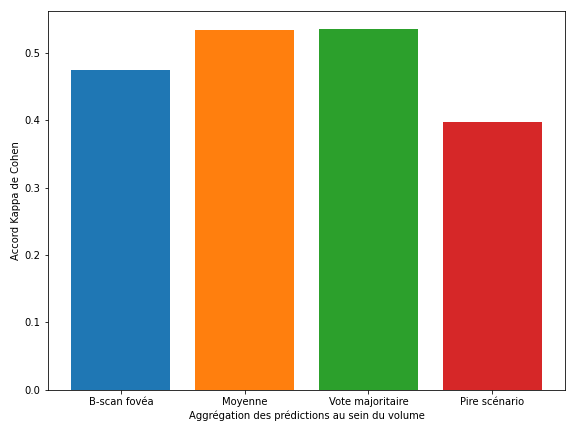
\includegraphics[width=.7\textwidth]{applications/DMLA/accord_selon_modalites}
	\caption{Accord au sens du $\kappa$ quadratique de Cohen entre les prédictions réalisées par le même réseau sur les images Zeiss ($6\times 6$mm$^2$) et Spectralis.}
	\label{fig:DMLA_accord_model_zeiss_spectralis}
\end{figure}
Quelles que soient les performances de généralisation, ajoutons que la prédiction en classes telles que \og Drusen\fg ou \og Néovascularisation\fg est une forte limitation à l'utilisation du modèle, notamment car ces symptômes ne sont pas mutuellement exclusifs. Par ailleurs, un B-scan peut aussi bien contenir peu que de nombreux drusens, ce qui change significativement le diagnostic. Une seule classe pour représenter cette diversité est donc une forte limitation. Malheureusement, cette contrainte nous vient des données à notre disposition.

\begin{figure}[!ht]
	\centering
	\begin{subfigure}{0.48\textwidth}
		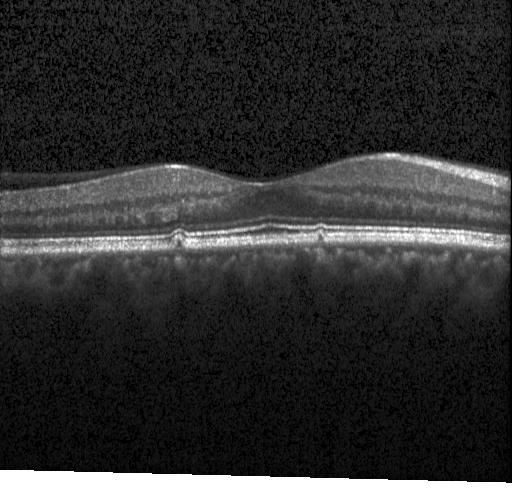
\includegraphics[width=\textwidth]{applications/DMLA/modality/UCSD}
		\subcaption{Image de la base UCSD, classe \og Drusen \fg}
	\end{subfigure}
\hfill
	\begin{subfigure}{0.48\textwidth}
		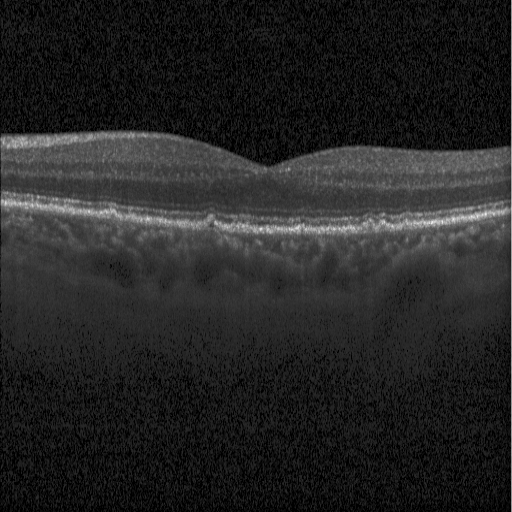
\includegraphics[width=\textwidth]{applications/DMLA/modality/oct}
		\subcaption{Cohorte HMR: Spectralis}
		\label{subfig:spectralis}
	\end{subfigure}
\hfill
	\begin{subfigure}{0.48\textwidth}
		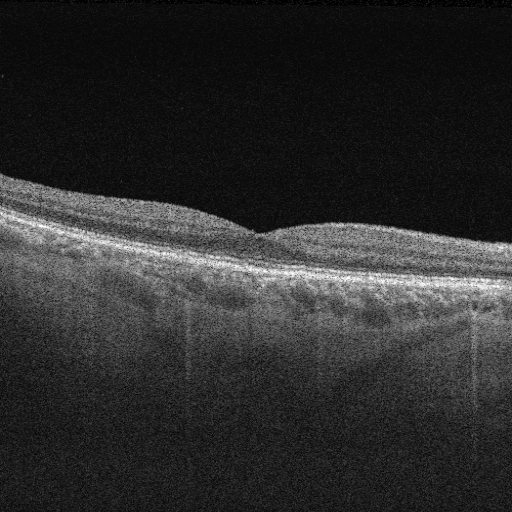
\includegraphics[width=\textwidth]{applications/DMLA/modality/zeiss_6mm}
		\subcaption{Cohorte HMR: Zeiss $6\times6$mm$^2$}
	\end{subfigure}
\hfill
	\begin{subfigure}{0.48\textwidth}
		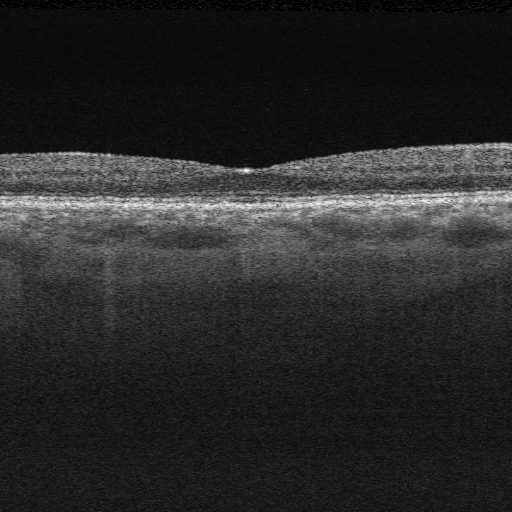
\includegraphics[width=\textwidth]{applications/DMLA/modality/zeiss_3mm}
		\subcaption{Cohorte HMR: Zeiss $3\times3$mm$^2$}
	\end{subfigure}
\caption{Acquisitions faites sur un même patient de la cohorte HMR comparées à un B-scan de la base publique UCSD sur laquelle sont entraînés nos modèles.}
\label{fig:IllustrationHMR_DMLA_modalities}
\end{figure}

\subsubsection{Utilisation des cartes d'interprétabilité}
Une alternative à l'utilisation des prédictions de classification repose sur la segmentation des structures pathologiques et leur suivi au cours du temps. L'avantage est de pouvoir dériver plusieurs scores (taille des structures, leur nombre, etc.) qui corrige les limitations des prédictions par image de la section précédente. De plus, ces scores sont également plus faciles à interpréter cliniquement.
Pour commencer, nous proposons d'utiliser les cartes d'attributions obtenues par les algorithmes d'interprétabilité, en particulier l'Attention Concentrée. Rappelons que celles-ci fournissent une indication approximative sur les structures locales qui ont guidé le diagnostic du modèle. La figure \ref{fig:DrusenDetectionWithFocusedAttention} fournit quelques exemples de drusens détectés par Attention Concentrée sur les patients de la cohorte. À chaque fois, nous avons extrait le B-scan central du volume Spectralis. Globalement, le modèle arrive à détecter correctement les drusens. Malheureusement, les indications fournies par la carte d'attribution restent peu précises: il ne s'agit pas d'une segmentation aux contours bien délimités qui permettrait de mesurer des statistiques de volume, largeur ou autres sur la lésion. Elles n'en restent pas moins utiles pour confirmer que le modèle n'hallucine pas lors de ses prédictions; mais en l'état, elles ne sont pas exploitables pour mesurer l'évolution des lésions. Pour s'en servir ainsi, une alternative possible est d'utiliser la carte d'attribution comme une forme d'initialisation ou de guidage pour un autre algorithme dédié lui à la segmentation et possiblement non supervisé, à l'instar d'un Watershed (Najman et Schmitt \cite{najmanWatershedContinuousFunction1994}). Nous n'avons pas expérimenté une telle approche qui reste donc ouverte à de futurs travaux.
\begin{figure}[!htb]
	\centering
	\includegraphics[width=0.9\textwidth]{applications/DMLA/attention_grid}
	\caption{Attention Concentrée calculée sur les patients de la cohorte DMLA. Chaque B-scan correspond à un patient différent et est diagnostiqué comme présentant des drusens par le modèle ViT.}
	\label{fig:DrusenDetectionWithFocusedAttention}
\end{figure}
 
\subsubsection{Classification de graphes de l'arbre vasculaire}
En s'appuyant sur les relatifs succès de la classification de graphes rétinien avec un GNN, nous nous sommes interrogé sur la viabilité de cette piste pour la classification de nos données d'OCT angiographiques. En effet, l'angiographie fournit une visualisation précise des vaisseaux et néo-vaisseaux à travers les différentes couches de la rétine. En particulier, la projection de ceux-ci dans le plan de la surface de la rétine (dite projection \og en-face \fg) fournit un arbre vasculaire similaire à celui visible dans le \fundus{} (mais nettement plus détaillé). Pour cela, une première étape nécessite à identifier les différentes couches rétiniennes, avant de pouvoir contrôler la profondeur de projection. Cette identification se fait donc via un premier modèle de segmentation. Là se ressent l'intérêt d'avoir les doubles modalités OCT structurelle et angiographiques calibrées entre elles: en effet, la segmentation des couches se fait dans la première et la projection de l'arbre vasculaire dans la seconde suivant la profondeur de la couche choisie. Nous avons donc entraîné un modèle de segmentation sur la base AROI publiée par Melinščak et al. \cite{melinscakAnnotatedRetinalOptical2021}. Cette segmentation est illustrée sur la figure \ref{fig:SegmentationAROI}. Outre diverses lésions, nous obtenons surtout les interfaces délimitant les couches rétiniennes.
\begin{figure}[!ht]
	\centering
	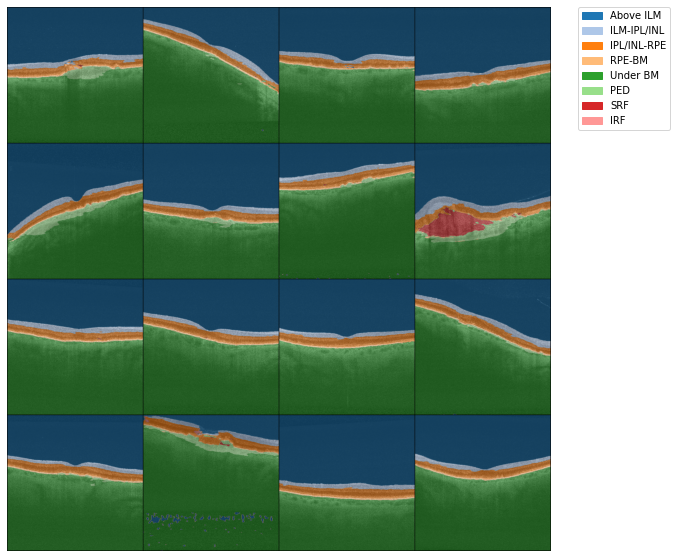
\includegraphics[width=\textwidth]{applications/DMLA/segmentation}
	\caption{Segmentation automatique des couches rétiniennes dans les images d'OCT structurelles. Chaque image de la mosaïque est prise sur un patient différent. \textit{ILM: Internal Limiting Membrane, IPL: Inner Plexiform Layer, INL: Inner Nuclear Layer, RPE: Retinal Pigment Epithelium, BM: Bruch Membrane, PED: Pigment Epithelial Detachment, SRF: Subretinal Fluid, IRF: Intraretinal Fluid}}
	\label{fig:SegmentationAROI}
\end{figure}
 
À partir des cartes de segmentation de chacune des couches, nous pouvons obtenir les projections vasculaires à différentes profondeurs. Une illustration en est donnée sur la figure \ref{fig:AngioOCTVascularTemporal}, représentant les acquisitions prises sur un même patient au cours de trois visites consécutives. À l'issue de la dernière, l'\oeil{} est diagnostiqué par un médecin comme présentant une forme de conversion (cependant le diagnostic n'est pas mené sur l'OCT angiographique mais bien structurelle). Notre objectif est bien de retrouver sur ces images un marqueur d'évolution qui correspond à cette progression de la maladie. Mais il est notable au premier coup d'\oeil{} que les images ne présentent pas de variations brutales au cours du temps: si marqueur il y a, celui-ci sera très certainement subtil et probablement à chercher au niveau des capillaires. Sans rentrer dans les détails méthodologiques, nous proposons d'analyser l'évolution topologique de l'arbre vasculaire. Pour cela, la première étape est d'en réaliser une segmentation et squelettisation. La forme squelettisée est propice pour une représentation sous forme de graphe du réseau vasculaire: chaque vaisseau et ses embranchements y représentent un sous-graphe. La représentation par graphe est particulièrement propice pour représenter l'apparition de nouveaux vaisseaux. En attachant à chaque arête des caractéristiques (par exemple, la tortuosité ou la longueur du vaisseau entre les deux \noeud{}s aux extrémités de l'arête en question), le graphe permet de modéliser finement l'état de l'arbre vasculaire.  L'évolution temporelle peut alors se faire en faisant une comparaison longitudinale de graphes. Une métrique de proximité entre graphes n'est pas triviale à définir mais une telle analyse est parfois faite à l'aide de GNN: cela correspond donc à une nouvelle application possible de l'architecture Attention-GNN développée dans le chapitre \ref{sec:ChapitreSegmentation}. 
\begin{figure}[!ht]
	\centering
	\begin{subfigure}{.9\textwidth}
		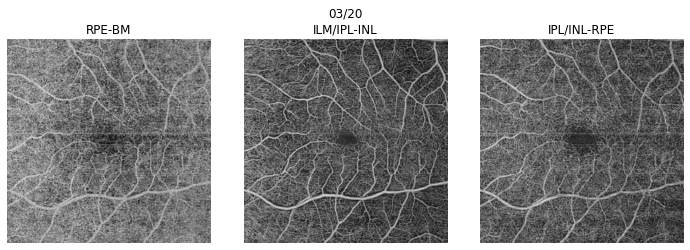
\includegraphics[width=\textwidth]{applications/DMLA/temporal_vasculature/1}
	\end{subfigure}
	\begin{subfigure}{.9\textwidth}
		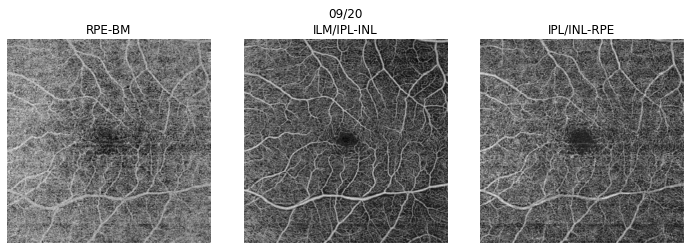
\includegraphics[width=\textwidth]{applications/DMLA/temporal_vasculature/2}
	\end{subfigure}
	\begin{subfigure}{.9\textwidth}
		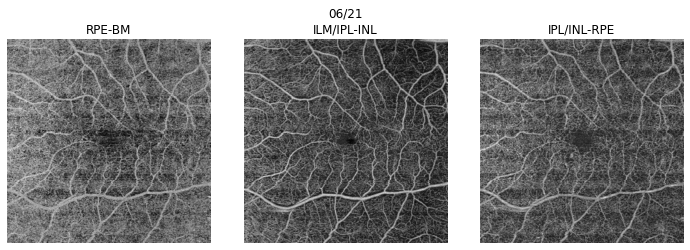
\includegraphics[width=\textwidth]{applications/DMLA/temporal_vasculature/3}
	\end{subfigure}
\caption{Évolution temporelle de l'arbre vasculaire d'un patient dont l'\oeil{} a subi une conversion vers une DMLA humide. Chaque projection vasculaire est réalisée à différentes profondeurs, obtenues grâce à la segmentation menée sur l'OCT structurelle correspondante.}
\label{fig:AngioOCTVascularTemporal}
\end{figure}

\section{Considérations sur un hypothétique déploiement clinique}
La précédente section a couvert une application potentielle de nos algorithmes, orientée autours de la DMLA. Ces travaux ont pour objectif la compréhension de l'évolution de la maladie et ont un intérêt surtout théorique. Dans cette section, c'est une autre application que nous souhaitons présenter, qui consiste au développement d'une plateforme d'aide au diagnostic clinique dans la pratique quotidienne. Cette plateforme peut aussi servir d'aide à la formation à la lecture d'images rétiniennes. C'est un un prototype (voire juste une preuve de concepts) que nous introduisons ici, visant à démontrer un usage et l'intérêt des algorithmes développés. Sans rentrer sur son développement technique, la plateforme proposée fonctionne sur navigateur, elle ne nécessite donc pas d'installation. Elle permet à l'utilisateur de choisir une image de \fundus{} à traiter (ou de parcourir la base de données d'images existantes). L'image est envoyée sur un serveur, sur lequel les algorithmes de segmentation et de classification par graphe sont déployés. Le serveur renvoie alors la réponse des modèles, comprenant le graphe rétinien et le score de gradation de la rétinopathie diabétique prédit. L'utilisateur peut alors visualiser ce que les modèles ont découvert dans l'image. Une double capture d'écran est présentée sur la figure \ref{fig:plateformeOutilsAlgo}: les fonctionnalités de la plateforme sont relativement sommaires, mais elle permet d'apprécier l'intérêt pratique de la classification par graphes. En effet, cette approche se prête bien à la visualisation de différentes statistiques globales: quantité de chacune des lésions, distribution des tailles etc. Un autre avantage de l'approche par graphe est sa rapidité d'exécution et le poids des modèles: comme nous l'avons vu, ces deux variables se comparent très favorablement aux CNNs conventionnels. Or, d'un point de vue technique, des modèles particulièrement légers permettent à terme un déploiement décentralisé directement dans le navigateur \footnote{En s'appuyant sur des technologies encore en développement telles que le standard inter-plateforme d'export de réseaux de neurones ONNX et le langage WASM.}. Cet aspect est particulièrement intéressant au regard de la confidentialité des données, une inférence dans le navigateur de l'utilisateur étant bien plus sécurisée que le transfert sur un serveur de calcul central. Bien que cet élément de discussion soit important, nous ne l'avons pas expérimenté sur notre plateforme. Pour être parfaitement complet, il faut aussi relever que même si le modèle de classification de graphes est léger, celui dédié à la segmentation ne l'est pas spécialement; d'importantes optimisations restent donc à faire pour aboutir à une inférence complètement décentralisée.
\begin{figure}[!htb]
	\centering
	\begin{subfigure}{\textwidth}
		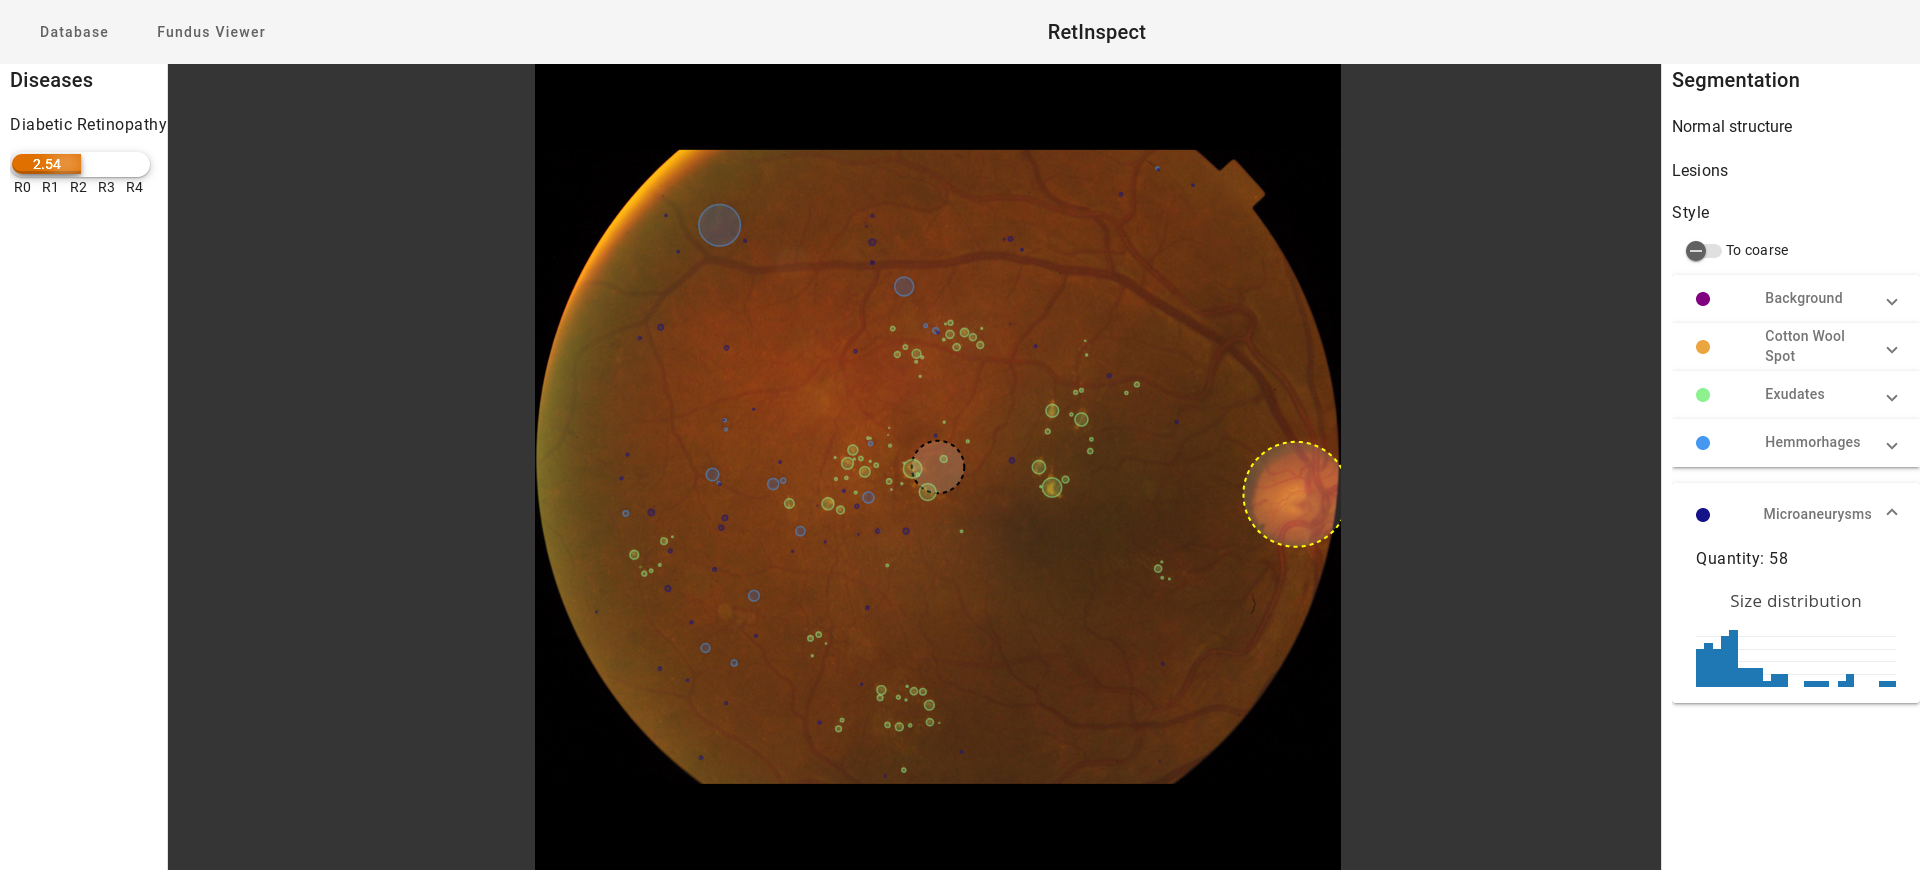
\includegraphics[width=\textwidth]{applications/Plateforme/screenshot1}
		\caption{Style de segmentation fin}
	\end{subfigure}
	\begin{subfigure}{\textwidth}

		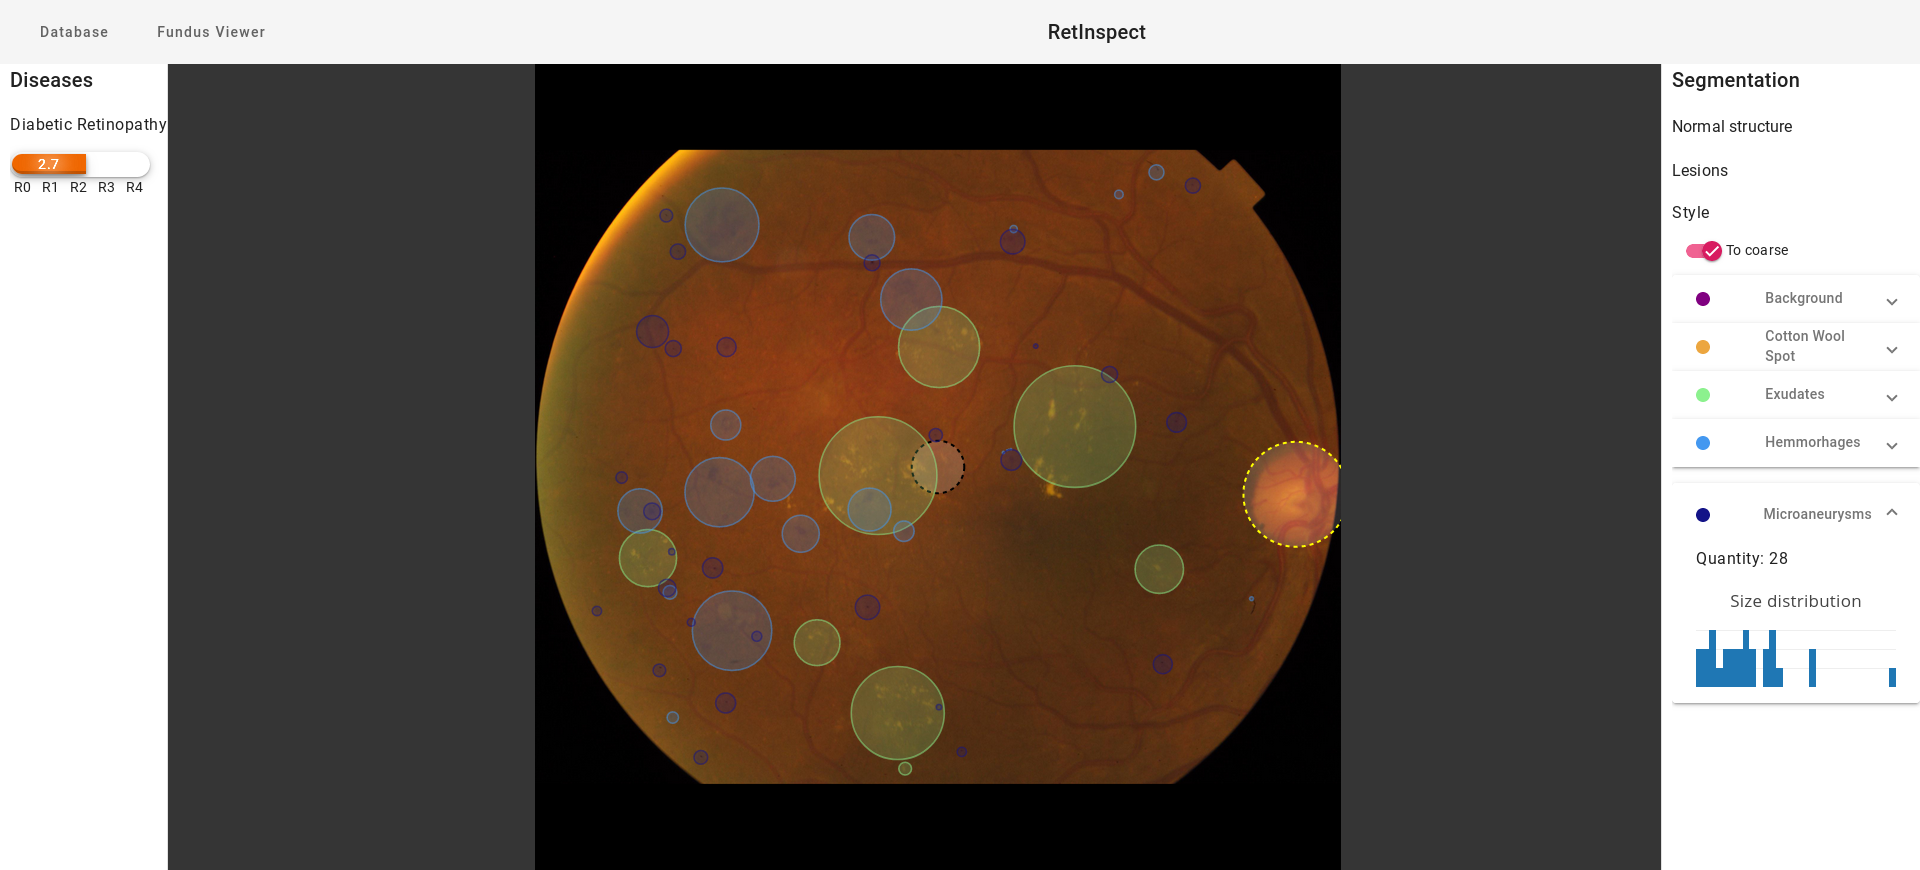
\includegraphics[width=\textwidth]{applications/Plateforme/screenshot2}
		\caption{Style de segmentation large}
	\end{subfigure}
\caption{Plateforme de visualisation des prédictions faites par nos modèles. L'utilisateur peut choisir de faire une conversion adversariale du style d'annotations, ce qui influe sur le diagnostic du modèle.}
\label{fig:plateformeOutilsAlgo}
\end{figure}
L'approche par graphe présente également un intérêt en terme d'interprétabilité des modèles. En effet, bien que nous n'ayons que survolé cet aspect dans nos expériences, il est possible de quantifier l'importance de chaque \noeud{} dans la prédiction du modèle, en utilisant peu ou prou les mêmes algorithmes d'attributions locales que pour un CNN. Intrinsèquement, attribuer un score d'importance à un \noeud{} n'a d'utilité que si ce dernier est facilement visualisable. En ce sens, nous arguons que la notion d'interprétabilité ne peut pas se décorréler de l'outil mis à disposition de l'utilisateur pour l'appréhender. Notre prototype de plateforme répond justement à cette problématique: l'importance de chaque \noeud{} s'obtient simplement via une fenêtre qui apparaît en le survolant de la souris. La figure \ref{fig:ImportanceNoeudPlateforme} illustre ce concept: en plus du score d'importance à la classification, d'autres statistiques sont fournies, comme la taille de la lésion considérée ou sa distance à la fovéa (indiquée en pixels ou en fraction de diamètre de disque optique). Cependant, nous notons qu'une étude reste à mener auprès de la communauté médicale pour déterminer quels indicateurs sont les plus pertinents et facilitent le diagnostic de l'image. 
\begin{figure}[!h]
	\centering
	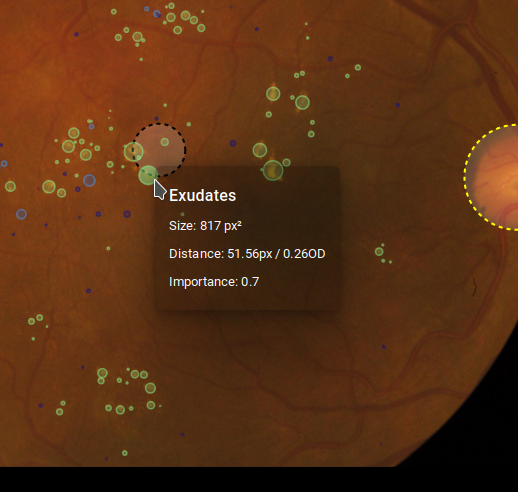
\includegraphics[width=.6\textwidth]{applications/Plateforme/screenshot3}
	\caption{Illustration de l'importance d'un \noeud{} dans la classification du graphe rétinien et autres statistiques associées consultables par l'utilisateur.}
	\label{fig:ImportanceNoeudPlateforme}
\end{figure}
Enfin, cette plateforme permet aussi prendre la mesure des limitations de nos travaux sur la segmentation du \fundus{}. Tout d'abord, une segmentation automatique du disque optique et de la macula est clairement manquante: elles sont faites ici manuellement. De manière générale, il semble clair que l'ajout de biomarqueurs plus précis, que ce soient d'autres classes de lésions ou qu'ils soient non pathologiques (arbre vasculaire, nerf optique, fovéa) devrait affiner la représentation par graphe de la rétine et potentiellement améliorer sa classification. Au delà des structures locales manquantes, nous pouvons également ajouter que la classification à la seule rétinopathie diabétique est une limitation importante quant à l'intérêt des algorithmes. Bien qu'encore peu nombreuses, plusieurs recherches démontrent l'intérêt d'étendre la classification à d'autres maladies et des bases de données consacrées à cette tâche commencent à voir le jour (voir par exemple Panchal et al \cite{panchalRetinalFundusMultiDisease2023}). 



